\documentclass[12pt]{article}

\usepackage[margin=1in]{geometry}
\usepackage{graphicx}
\usepackage[export]{adjustbox}
\usepackage[title,titletoc]{appendix}

\usepackage{amssymb,amsmath}
\usepackage{hyperref}
\usepackage{xcolor}

\usepackage{tabularx}
\usepackage{cleveref}
\usepackage{ltablex}
\usepackage{alltt}
\usepackage{listings}
\usepackage{enumitem}

\definecolor{InternalLinkColor}{HTML}{282888}
\definecolor{ExternalLinkColor}{HTML}{3333BB}

\hypersetup{
  colorlinks=true,
  linkcolor=InternalLinkColor,
  urlcolor=ExternalLinkColor
}

\definecolor{light-gray}{gray}{0.95}

\lstdefinelanguage{ir}
{
  backgroundcolor=\color{light-gray},
  morekeywords={version, circuit, public_input, private_input, configuration, field, @field, ext_field, ring, @begin, @end, @function, @out, @in, @public, @private, @call, @anon_call, @type, @plugin},
  morekeywords=[2]{@add, @addc, @mul, @mulc, @assert_zero, @delete, @convert, @new},
  keywordstyle={[2]\it},
  morecomment=[l]{//}
}

\lstdefinelanguage{flatbuffer}
{
  backgroundcolor=\color{light-gray},
  morekeywords={table,struct,union},
  morekeywords=[2]{uint32,uint64,ubyte,string},
  keywordstyle={[2]\it}
}

\lstdefinelanguage{json}{
    backgroundcolor=\color{light-gray},
    basicstyle=\ttfamily\small,
}

\lstset{escapechar=\#}

\definecolor{SyntaxGreen}{HTML}{116611}
\definecolor{SemanticPurple}{HTML}{550077}

\renewcommand{\familydefault}{\sfdefault}

\title{Introduction to the SIEVE Intermediate Representation}
\author{See Section \ref{contributors} for list of \nameref{contributors}}
\date{Last Updated: 2023-07-17}

\newcommand{\maxfieldcount}{256}

\begin{document}
\maketitle

\textbf{Distribution Statement ``A'':} Approved for Public Release, Distribution Unlimited.\\

This material is based upon work supported by DARPA under Contracts No.~HR001120C0087, HR001120C0086, HR001120C0085 and Agreement No.~HR00112020021.  Any opinions, findings and conclusions or recommendations expressed in this material are those of the author(s) and do not necessarily reflect the views of DARPA.

\section*{Identification and History}\label{history}

\begin{tabularx}{\textwidth}{|p{1in}|p{1in}|p{4in}|}
  \hline
  \textbf{Version} & \textbf{Date} & \textbf{Notable Changes}                                                                                                                                                                   \\
  \hline
  0.1.0            & 2020-09-19    & Initial version as proposed jointly by WizKit and FROMAGER teams on DARPA SIEVE.                                                                                                           \\
  \hline
  0.1.1
                   & 2020-12-16    & A number of bugfixes on the prior version.
  \begin{itemize}
    \item Fix typographical errors and omissions.
    \item Add checks for matching header, \texttt{num\_wires}, and etc., across multiple resources.
    \item Eliminate unused type-checking and arity-checking attributes from the attribute grammar, because IR0 has only one meaningful type.
    \item Add \texttt{num\_wires} to the instance and witness in the text and binary grammars.
  \end{itemize}                                                                                       \\
  \hline
  0.2.0            & 2021-03-19    & Remove the \texttt{num\_wires} and associated input size data and add a \texttt{@delete} directive.                                                                                        \\
  \hline
  1.0.0            & 2021-07-20    & Add ``uniformity'' features: function gates, public-index for loops, and private-condition switch-case statements.                                                                         \\
  \hline
  1.0.1            & 2022-04-29    & Fix the following issues:
  \begin{itemize}
    \item Fix switch-statement semantics which required a nested switch-statement where the outer case is inactive and the inner switch-statement has no active branch to cause an unexpected witness-statement invalidity.
    \item Constrain for-loop bounds and wire-ranges such that the first must be less than or equal to the last iteration or wire.
    \item Add a warning that the switch-statement conversion algorithm may produce a poorly-formed relation with certain forms of switch-statement and for-loop nesting. Add a suggestion to unroll for-loops in those conditions.
    \item Assorted typo fixes and performance improvements.
  \end{itemize} \\
  \hline
  2.0.0            & 2022-11-08    & The 2.0.0 revision is a significant departure from prior revisions, regressing some of the haphazardly developed high level features and preparing for the development of a distinct high-level (translation), and low-level (circuit) IR layers.
  This release was used during the SIEVE Phase II testing event, and specifies the Circuit-IR -- characterized as follows.
  \begin{itemize}
    \item Flat circuit with numbered wires.
    \item Function's encapsulating circuit fragments.
    \item Explicit allocation directives enable memory efficiency.
    \item A new plugin system allows access to backend-defined functionality.
  \end{itemize} \\
  \hline
  2.1.0            & 2023-07-17    & Adds ring and extension field types to the Circuit-IR and multi-wire convenience modes for copy gates and input gates. \\
  \hline
\end{tabularx}

\newpage
\tableofcontents
\newpage

%%%%
\section{Introduction}\label{sec:intro}

This document specifies the current version of the SIEVE Intermediate Representation (IR).
 Throughout the DARPA SIEVE program, changes to this specification were to be discussed and modified only through the decision process outlined in the \href{https://docs.google.com/document/d/1imP-9fXy8fQwr1e6ZEuhHnVDGkh1YdUOjEd1ifas6IM/edit?ts=5f614241&pli=1}{SIEVE IR Agreement document}.
The IR's developers are currently seeking a venue to host further development and standardization after the SIEVE program ends.
\\

The IR is an interaction between the front-end and the back-end portions of a Zero Knowledge (ZK) proof pipeline.
The frontend transforms high level statements in a target domain into the IR.
It is the producer of the three resources which are the subject of this document.
The backend is the consumer of them: it is an interaction between a Prover and a Verifier, where the Prover wishes to prove a statement to the Verifier, without revealing a secret component of the proof.
The primary goal for this specification is to define a standard format for ZK statements, so that there is interoperability between multiple frontends and backends.
\\

At a high level, ZK proofs involve three resources provided by the frontend and used by the backend as the fact being proven.

\begin{itemize}
  \item Relation -- a mathematical relationship between the inputs.
  \item Public inputs -- inputs to the relation given to both the Prover and Verifier.
  \item Private inputs -- inputs to the relation given only to the Prover.
\end{itemize}

\noindent 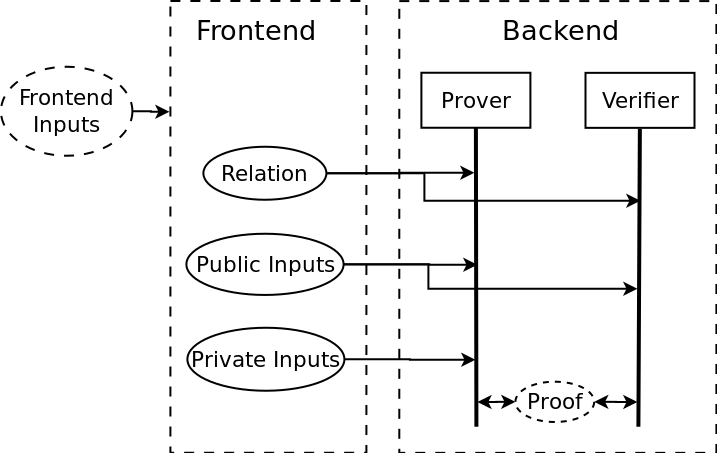
\includegraphics[width=0.75\textwidth,center]{ir-dataflow-simple.png} \\

\subsection{Genesis}

In the course of the SIEVE Program, performers experimented with a variety of representations ranging from very high level through very low level.
The SIEVE Program has proved statements on every platform from mobile web to gigantic cloud instances, with runtime taking anywhere from milliseconds to days to prove.
Additionally, SIEVE backends have preferred a wide variety of intermediate representations -- including R1CS, C++ compilation, and other custom solutions.
The greatest challenge in developing the IR has been making it flexible enough to accomodate so many requirements.

The program's first attempt at a flexible IR, the SIEVE IR v1.0, was to essentially overlay high-level features upon a flat circuit with numbered wires.
This was a failure for backends wanting just flat circuits because they were forced to unroll high level features.
It was also a failure for the higher level backends because the numbered wires were insufficient to convey high level meaning and long stretches of flat circuitry would cause slowdowns for them.

\subsection{Flexibility and Scalability}

To resolve this issue, the latest SIEVE IR revision has two layers.
The lower layer, called the Circuit-IR, defines a flat circuit, augmented with flat functions.
While it is not completely flat, it does strike a balance between statement size and interpreter complexity -- important because many SIEVE backends bottlenecked on disk IO while reading completely flat circuits.

A great strength of the Circuit-IR is circuit streaming.
Gates are processed one after the other, and their outputs (wires) are stored until needed for further computation.
Ordinarily, this would cause memory usage to increase until either the circuit ends or the available memory is exhausted.
The Circuit-IR implements memory management operations and restrictions which enables a circuit to declare what wires it will produce and when it is finished with them, so that its memory may be recycled.

The higher layer, called Translation-IR, is a fairly high level language in terms of control flow.
For maximal compatibility, SIEVE Performers are also developing a translation into the Circuit-IR, hence the name Translation-IR.
But the Translation-IR need not be translated just to the Circuit-IR, one of its goals is that it be translatable to non-SIEVE IRs such as the aforementioned R1CS, C++ compilation, or other custom solutions.
At the time of writing, the Circuit-IR recently survived the program's Phase II Testing Event, while the Translation-IR is currently in development.

\subsection{Multi Field Circuits}
To most practitioners of ZK, a single prime field is chosen at the beginning of a proof and used throughout.
However, for some applications it is desirable to use multiple primes for different elements within a single larger proof.
For example a large and expensive prime may be needed to verify public-key signatures, while a medium sized prime is necessary for large scale business logic.

To accommodate these applications, the IR must allow for multiple fields within a single relation.
To the frontend each field must describe the type of a wire, while to the backend these wires actually belong to multiple independent proofs.
An analogy to the real world might be a circuit card with transistor logic on one side and high voltage on the other.

Occasionally information from one field will be required in another.
The IR models this using a conversion gate with inputs in one field and outputs in another.
To continue the analogy, a relay would allow information to flow from transistor logic into high voltage, or in reverse, an analog-digital converter.
In ZK, methodologies must be developed and used to show equivalence of inputs and outputs across independent proofs or even across different proof systems.

\subsection{Resources of the SIEVE IR}
Each file or connection in the SIEVE IR is referred to as a resource, a stream of bytes to be consumed by the backend.
A relation is a resource, and so are the inputs to the relation.
There is also a special configuration resource which helps frontends and backends negotiate compatibility.

The SIEVE IR introduces two types of relation: the Circuit-IR and the Translation-IR.
\begin{itemize}
\item The Circuit-IR is defined by flat lists of gates and wires; functions may be defined and reused within the circuit.
\item The Translation-IR is a program which outputs a relation in the Circuit-IR format.
The backend is given some amount of control over how the Translation-IR is translated, and is free to reimplement common or standardized libraries, translate to an alternative IR, or even prove statements directly from the Translation-IR.
\end{itemize}

In recognition that many ZK backends can improve upon simple circuits' performance when particular functionality is desired, both layers of the IR define a \textbf{plugin} interface allowing calls from the IR into backend specific functionality.\\

To ease the frontends choice of configuration constants (such as prime fields and plugin parameters), a Circuit Configuration Communication occurs so that the backend may feed optimal constants to the frontend. \\

In total, the IR winds up with five resources: four in the frontend to backend direction, and a configuration which flows in the opposite direction.

\begin{itemize}
  \item Relation
  \begin{itemize}
     \item Translation-IR -- high level program which emits a flat circuit
     \item Circuit-IR -- flat circuit which is easy for backends to ingest
  \end{itemize}
  \item Public inputs -- a list of inputs known to both the Prover and Verifier
  \item Private inputs -- a list of inputs known only to the Prover
  \item Circuit Configuration Communication (CCC) - hints from the backend to the frontend describing features supported by the backend.
\end{itemize}

This illustration shows how the backends start by producing the CCC -- typically checked in with its source code -- enabling a frontend to choose types and plugins suitable to a backend.
Then the frontend can produce SIEVE IR enabling a web of available translations before the backend can finally prove the statement.

\noindent 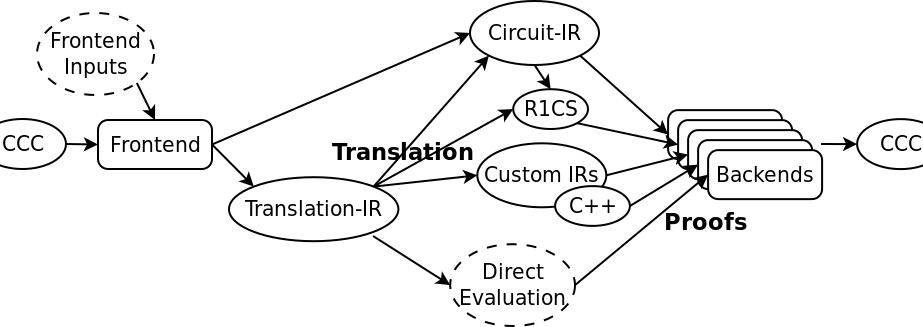
\includegraphics[width=0.95\textwidth,center]{ir-dataflow-translation.png} \\

%%%%
\section{Headers}
\label{sec:headers}

All SIEVE IR files start with a header.
The header contains % the following parameters:
a version number for quick recognition of the IR
and
a resource type.
Each resource type may define additional header declarations that appear after the version and resource type, but before the \texttt{@begin} keyword.

\begin{description}
  \item[\texttt{circuit}] Circuit-IR
  \item[\texttt{translation}] Translation-IR
  \item[\texttt{public\_input}] Public input streams (the \textit{instance})
  \item[\texttt{private\_input}] Private input streams (the \textit{witness})
  \item[\texttt{configuration}] the Circuit Configuration Communication
\end{description}

%
Here is an example header.
\begin{lstlisting}[language=ir]
version 2.0.0;
private_input;
\end{lstlisting}
This indicates the file is a private input resource for version 2.0.0 of the SIEVE IR.



%%%%
\section{Subdocuments of the SIEVE IR}
This spec is organized into multiple subdocuments.

\begin{itemize}
  \item The Circuit-IR document includes formats and semantics for the public and private input streams and the CCC.
  \item The Translation IR document is currently in development, and unreleased.
  \item the Plugins directory contains sub documents for each plugin which has been standardized (although backends are free to develop their own plugins).
\end{itemize}

%%%%

\section{Contributors}\label{contributors}

\paragraph{Authors}
\begin{itemize}
    \item Team Wizkit: Paul Bunn, David Darais, Daniel Genkin, Steve Lu, Kimberlee Model, Tarik Riviere, Muthuramakrishnan Venkitasubramaniam, Xiao Wang
    \item Team Emphasize:
    Steven Eker, Karim Eldefrawy, Stéphane Graham-Lengrand, Vitor Pereira, Hadas Zeilberger 
    \item Team Fromager: Michael Adjedj, Daniel Benarroch Guenun, Eran Tromer, Aurélien Nicolas, Constance Beguier, Alex Malozemoff, James Parker, Chris Phifer
    \item Team Oracles: Mayank Varia
\end{itemize}

The following individuals from the T\&E Team were instrumental in moderating the IR's development:
David A. Wilson (PI),
R. Nicholas Cunningham,
J. Parker Diamond,
Hanson Duan,
Ariel Hamlin,
Noah Luther,
Richard Shay.\\

\noindent\textbf{Disclaimers}
\\

\textbf{Distribution Statement ``A'':} Approved for Public Release, Distribution Unlimited. \\

This material is based upon work supported by DARPA under Contracts No.~HR001120C0087, HR001120C0086, HR001120C0085 and Agreement No.~HR00112020021.  Any opinions, findings and conclusions or recommendations expressed in this material are those of the author(s) and do not necessarily reflect the views of DARPA.\\

The authors of the SIEVE IR have made every effort that the SIEVE IR Specification, if adopted by a recognized standards body, would be compatible with \href{https://opensource.org/osr}{the OSI Open Standard Requirement}.

\begin{description}
  \item[No Intentional Secrets] We have made every effort to ensure that the IR contains no necessary secrets. Further, several of the SIEVE Performers have or will open-source their IR implementations.
  \item[Availability] The SIEVE Performers have agreed to release the text of the IR Specification under the \href{https://creativecommons.org/licenses/by/4.0/}{Creative Commons Attribution 4.0 International (CC-BY 4.0)} terms.
  \item[Patents] Although we are not aware of any current patents which may be necessary to implement the IR, the SIEVE Performers have \href{https://github.com/sieve-zk/ir/raw/main/v1.0.1/release_acknowledgments.pdf}{agreed not to enforce} any intellectual property rights which may be necessary to implement the IR.
  \item[Dependencies] To our knowledge, all technologies dependent by the IR are already themselves open-source.
\end{description}


\end{document}
